% Stage 4: final project report, written as a summary of the whole project.
% Compile from this folder: pdflatex stage4_Kai.tex (twice).
\documentclass[11pt,a4paper]{article}
\usepackage[margin=2.2cm]{geometry}
\usepackage[T1]{fontenc}
\usepackage{lmodern}
\usepackage{amsmath}
\usepackage{graphicx}
\usepackage{booktabs}
\usepackage{array}
\usepackage{enumitem}
\usepackage{xcolor}
\usepackage{caption}
\usepackage[hidelinks]{hyperref}
\graphicspath{{../experiments/}}
\setlist{itemsep=1pt,topsep=3pt}
\setlength{\parindent}{0pt}
\setlength{\parskip}{4pt}
\captionsetup{font=small,labelfont=bf}
\newcommand{\us}{\,$\mu$s}
\newcommand{\degC}{\,\textdegree C}
\newcommand{\todo}[1]{\textcolor{red}{[TODO: #1]}}

\begin{document}

\begin{center}
{\LARGE\bfseries Lightweight Temperature Predictor:\\[2pt] TapaSense}\\[8pt]
Ethan Bobby Kurien \quad Kaivalya Mase
\end{center}

\begin{abstract}
Dynamic thermal management (DTM) needs core temperatures every millisecond, and ideally a few
milliseconds ahead. The HotSpot simulator computes them accurately but needs 0.24\,s per steady
answer and 5.5\,ms per 1\,ms transient step. We built a two-stage predictor for heterogeneous
multicore floorplans. A one-time calibration runs HotSpot 8 times (steady) or 24 times (steady and
transient) per floorplan with 1\,W in one core at a time. The prediction stage then uses only the
stored coefficients. Because HotSpot without leakage is linear, the steady predictor (an influence
matrix) is exact to HotSpot's printed precision ($3\times10^{-5}$\,K worst) at 2.6\us\ per
prediction from under 1\,kB. The transient predictor (a sum of four exponentials per pair of
cores) is within 0.06--0.09\,K on average and 0.3\,K worst, at 3\us\ per step from about 4\,kB.
Every calibration-free alternative is 0.5--2.7\,K off on average.
\end{abstract}

\tableofcontents

%=====================================================================
\section{Introduction}
A modern chip has several cores. Under load they heat up, and above a limit they slow down, age
faster or fail. The chip's DTM software throttles cores to stay under the limit. To act before the
limit is crossed it needs fast predictions of temperature.

\textbf{Problem statement.} Develop a lightweight temperature predictor in two stages.
Calibration (one-time per floorplan): tune predictor coefficients for the given floorplan with
heterogeneous cores. Prediction: predict the temperature (steady state or transient) for a given
power input. Metrics: accuracy, prediction time, model size. Wishlist: show the effectiveness of
the predictor for proactive DTM.

\textbf{Contributions.}
\begin{itemize}
  \item A calibration stage of 8 (steady) or 24 (steady and transient) planned HotSpot runs per
        floorplan.
  \item An exact steady predictor and an accurate transient predictor, each compared against
        simpler and calibration-free alternatives.
  \item A Python tool (\texttt{ltp}) for both stages, built on a patched HotSpot (6-decimal output,
        29$\times$ faster transients with identical output, a memory-leak fix).
\end{itemize}

%=====================================================================
\section{Background}
\textbf{HotSpot} \cite{hotspot} models the die and package (silicon, thermal interface, heat
spreader, heat sink) as a network of thermal resistances and capacitances. The grid model divides
the die into cells (here $64\times64$); the block model uses one node per block and is faster but
1--5\,K off on our floorplans \cite{hotspot4}.

\textbf{Linearity.} Without temperature-dependent leakage the network is linear, so rises scale
with power and add up across cores; we confirmed this to $10^{-6}$\,K. Then
$T = T_\text{amb} + G\,P$ in steady state, where $G_{ij}$ is the rise of block $i$ per watt in
core $j$.

%=====================================================================
\section{Design approach}

\subsection{Two stages}
\begin{description}[leftmargin=1.2em]
  \item[Calibration] (once per floorplan): $N$ steady runs with 1\,W in core $j$ give column $j$ of
        $G$. $N$ short step runs (1\,ms sampling for 2\,s) and $N$ long step runs (20\,ms sampling
        for 100\,s) give the step response $s_{ij}(t)$ of every block to every core. For $N=8$ that
        is 24 runs.
  \item[Prediction] (many times): load the model file (about 8\,kB), give the power per core, get
        every block's temperature now (steady) or over time (transient).
\end{description}

\subsection{Models used}
\textbf{Steady state: influence matrix.} $G[:,j] = T_\text{HotSpot}(\text{1\,W in core } j) -
T_\text{amb}$, and $T = T_\text{amb} + G P$. No fitting is involved.

\textbf{Hot spots: influence matrix on candidate cells.} Core averages hide hot spots inside a
core. From the same runs' $64\times64$ maps we keep, for each core, the 3--9 cells that were its
hottest point in any calibration run or at nominal power, and predict
$T_\text{hot}(c) = \max_{q} (T_\text{amb} + G^\text{cell}_{q\cdot} P)$.

\textbf{Transient: sum of exponentials.} Each step response is fitted as
$s_{ij}(t) \approx \sum_{m=1}^{M} a_{ijm}(1-e^{-t/\tau_m})$, with time constants $\tau_m$ shared
by all pairs and $\sum_m a_{ijm} = G_{ij}$. At run time, with $\lambda_m = e^{-\Delta t/\tau_m}$:
\begin{equation}
  z_{jm}[k+1] = \lambda_m z_{jm}[k] + (1-\lambda_m) P_j[k],
  \qquad T_i = T_\text{amb} + \sum_{j,m} a_{ijm} z_{jm}[k+1].
\end{equation}

\subsection{Evaluation}
\begin{itemize}
  \item Reference: HotSpot grid $64\times64$, the given layer stack, HotSpot's example package,
        ambient 45\degC, $\Delta t = 1$\,ms.
  \item Test inputs are never used for calibration: nominal and maximum power and 300 random power
        vectors per floorplan (steady); random phase traces of 2\,s and 10\,s (transient).
  \item Accuracy: mean and worst absolute error over cores, and the share of cases with the right
        hottest core. Time: median of 10{,}000 single calls, one thread. Size: stored coefficients
        $\times$ 8 bytes.
\end{itemize}

%=====================================================================
\section{Data}
\begin{center}
\small
\begin{tabular}{@{}l p{8.5cm} c@{}}
\toprule
Set & Description & Floorplans \\
\midrule
Given floorplans & 2 big (4$\times$4\,mm) + 6 little (2$\times$2\,mm) cores, 4 styles & 23 \\
Generated & Our generator, 13 per style of the given floorplans & 52 \\
Many-core & Grid of 64 identical cores (compression test) & 1 \\
\bottomrule
\end{tabular}
\end{center}
Power: nominal big 20\,W and little 8\,W (88\,W per chip); random vectors with big 10--20\,W and
little 5--10\,W; phase traces where every core switches between 4 levels with phases from 1\,ms to
2\,s. At nominal power the given floorplans reach 69--77\degC, and a little core is always the
hottest.

%=====================================================================
\section{Calibration}
Calibrating one floorplan takes 24 HotSpot runs; the steady model alone needs 8 runs (4.3\,s). The step responses contain time constants from about 1\,ms to 8\,s, so a single
time constant cannot fit them, and four can (Figure~\ref{fig:steps}). A little core heats itself
2.4$\times$ as much per watt as a big core.

\begin{figure}[h]
  \centering
  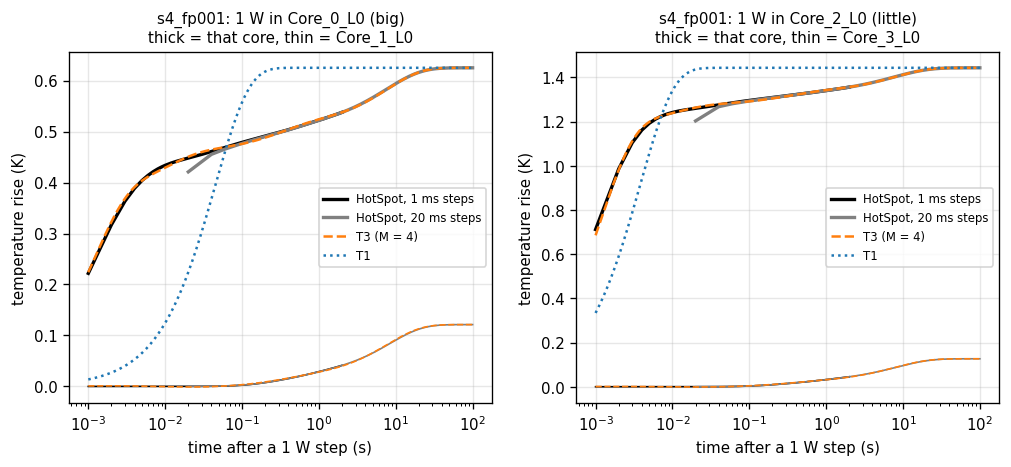
\includegraphics[width=0.85\linewidth]{P1-1_step_calibration/results/step_response_fits.png}
  \caption{Step responses to 1\,W in a big core (left) and a little core (right). HotSpot and the
  sum of four exponentials overlap; a single time constant has the right final value but the wrong
  shape.}
  \label{fig:steps}
\end{figure}

\textbf{Is calibration needed?} Yes. On 6{,}946 unseen runs, every way of predicting without runs
on the target floorplan is far worse than the calibrated influence matrix:
\begin{center}
\small
\begin{tabular}{@{}l c c c c@{}}
\toprule
Method & Runs on target & Mean & Worst & Hottest core right \\
\midrule
\textbf{Calibrated influence matrix} & 8 & 0.000007\,K & 0.00003\,K & 100\,\% \\
Power blurring \cite{blurring} + learned correction & 0 & 0.55\,K & 3.4\,K & 80\,\% \\
Power blurring & 0 & 0.76\,K & 5.2\,K & 71\,\% \\
Borrow a similar floorplan's $G$ & 0 & 1.11--2.66\,K & 5.2--12.1\,K & 45--60\,\% \\
One model per core type & 0 & 1.34\,K & 8.3\,K & 61\,\% \\
Regression on geometry & 0 & 1.94\,K & 7.4\,K & 42\,\% \\
\bottomrule
\end{tabular}
\end{center}
Even floorplans of the same style, where only the core positions differ, cannot share a model:
edges, distances and die size make each $G$ unique.

Calibrating from one recorded trace instead (an ARX model) needs a trace of at least 5\,s, is
3--5$\times$ less accurate than the planned step runs, and can be unstable.

%=====================================================================
\section{Steady-state results}
\begin{center}
\small
\begin{tabular}{@{}l c c c c c@{}}
\toprule
Model (24 floorplans) & Mean & Worst & Time & Size & vs HotSpot \\
\midrule
\textbf{Influence matrix} & 0.000006\,K & 0.00003\,K & 2.6\us & 928\,B & 91{,}000$\times$ faster \\
Influence matrix, 32-bit & 0.000006\,K & 0.00003\,K & 3.1\us & 464\,B & 77{,}000$\times$ \\
Power blurring (no calibration) & 0.77\,K & 5.2\,K & 2.5\us & 928\,B & 94{,}000$\times$ \\
\bottomrule
\end{tabular}
\end{center}
Batching 302 inputs per call brings the cost to 0.06\us\ per prediction. For chips with many
cores, keeping only the nearest neighbours' entries shrinks $G$ on a 64-core grid from 32.8\,kB to
5.7\,kB at 0.59\,K worst.

\textbf{Hot spots.} The hottest cell is 3--9\,K above its core's average, and it moves with the
power pattern in 61\,\% of cases, so a fixed offset cannot capture it:
\begin{center}
\small
\begin{tabular}{@{}l c c c c@{}}
\toprule
Hot-spot model & Size & Mean & Worst & Hottest core right \\
\midrule
Core average & 512\,B & 2.73\,K & 8.96\,K & 50\,\% \\
Core average + fixed offset & 576\,B & 0.59\,K & 4.11\,K & 82\,\% \\
\textbf{Candidate cells} & 3.1\,kB & 0.078\,K & 1.6\,K & 90\,\% \\
All cells (exact) & 115\,kB & 0.000007\,K & 0.00003\,K & 100\,\% \\
\bottomrule
\end{tabular}
\end{center}

%=====================================================================
\section{Transient results}
\begin{center}
\small
\begin{tabular}{@{}l c c c c@{}}
\toprule
Model (24 floorplans, 2\,s traces) & Mean & Worst & Time per step & Size \\
\midrule
One time constant per block & 7.25\,K & 14.6\,K & 1.5\us & 1.0\,kB \\
ARX fitted to one trace \cite{coskun,singla} & 0.19\,K & 0.57\,K & 5.4\us & 6.2\,kB \\
\textbf{Sum of exponentials, $M=4$} & 0.090\,K & 0.30\,K & 3.1\us & 3.7\,kB \\
Sum of exponentials, $M=6$ & 0.0093\,K & 0.13\,K & 3.2\us & 5.6\,kB \\
HotSpot's network reduced to 32 states \cite{matex,sharifi08} & -- & 0.047\,K & -- & 16\,kB \\
\bottomrule
\end{tabular}
\end{center}
The sum of exponentials gives the best accuracy for its size from 2 to 6\,kB; HotSpot's own
network, exported and reduced, is better only from about 16\,kB. It also confirms the calibration
independently: its steady gain equals $G$.

\begin{figure}[h]
  \centering
  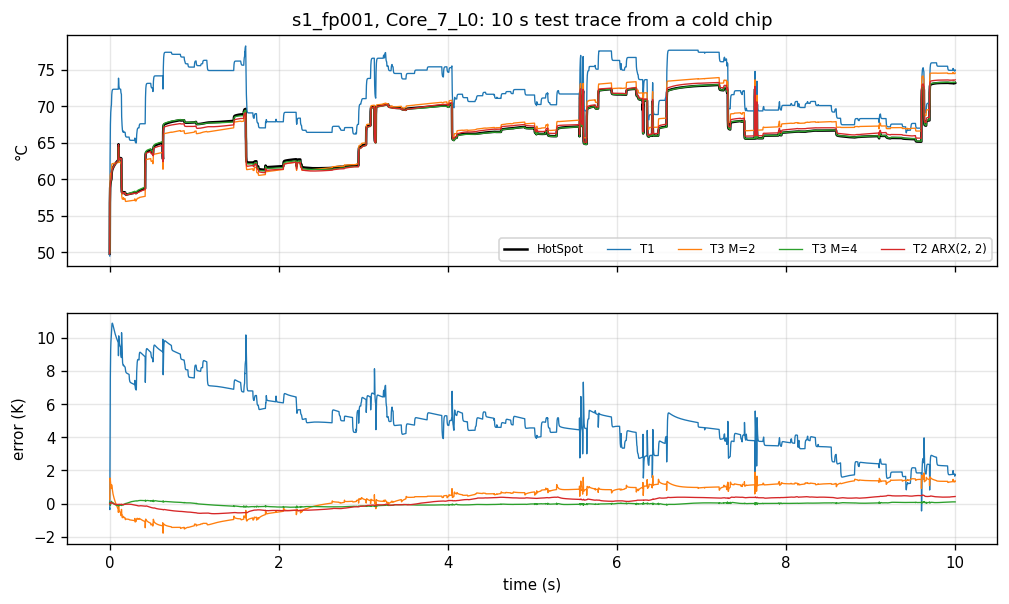
\includegraphics[width=0.6\linewidth]{P3-1_transient_predictor/results/trace_example.png}
  \caption{The transient predictor on a test trace, on top of HotSpot.}
\end{figure}

%=====================================================================
\section{Validation on 52 generated floorplans}
After the models were designed we generated 52 new floorplans in the styles of the given ones. The
results carry over:
\begin{center}
\small
\begin{tabular}{@{}l c c c c@{}}
\toprule
Set & Steady mean & Steady worst & Transient mean & Transient worst \\
\midrule
52 generated floorplans & $6.5\times10^{-6}$\,K & $3.4\times10^{-5}$\,K & 0.091\,K & 0.34\,K \\
24 given floorplans & $6\times10^{-6}$\,K & $3\times10^{-5}$\,K & 0.090\,K & 0.30\,K \\
\bottomrule
\end{tabular}
\end{center}

\begin{figure}[h]
  \centering
  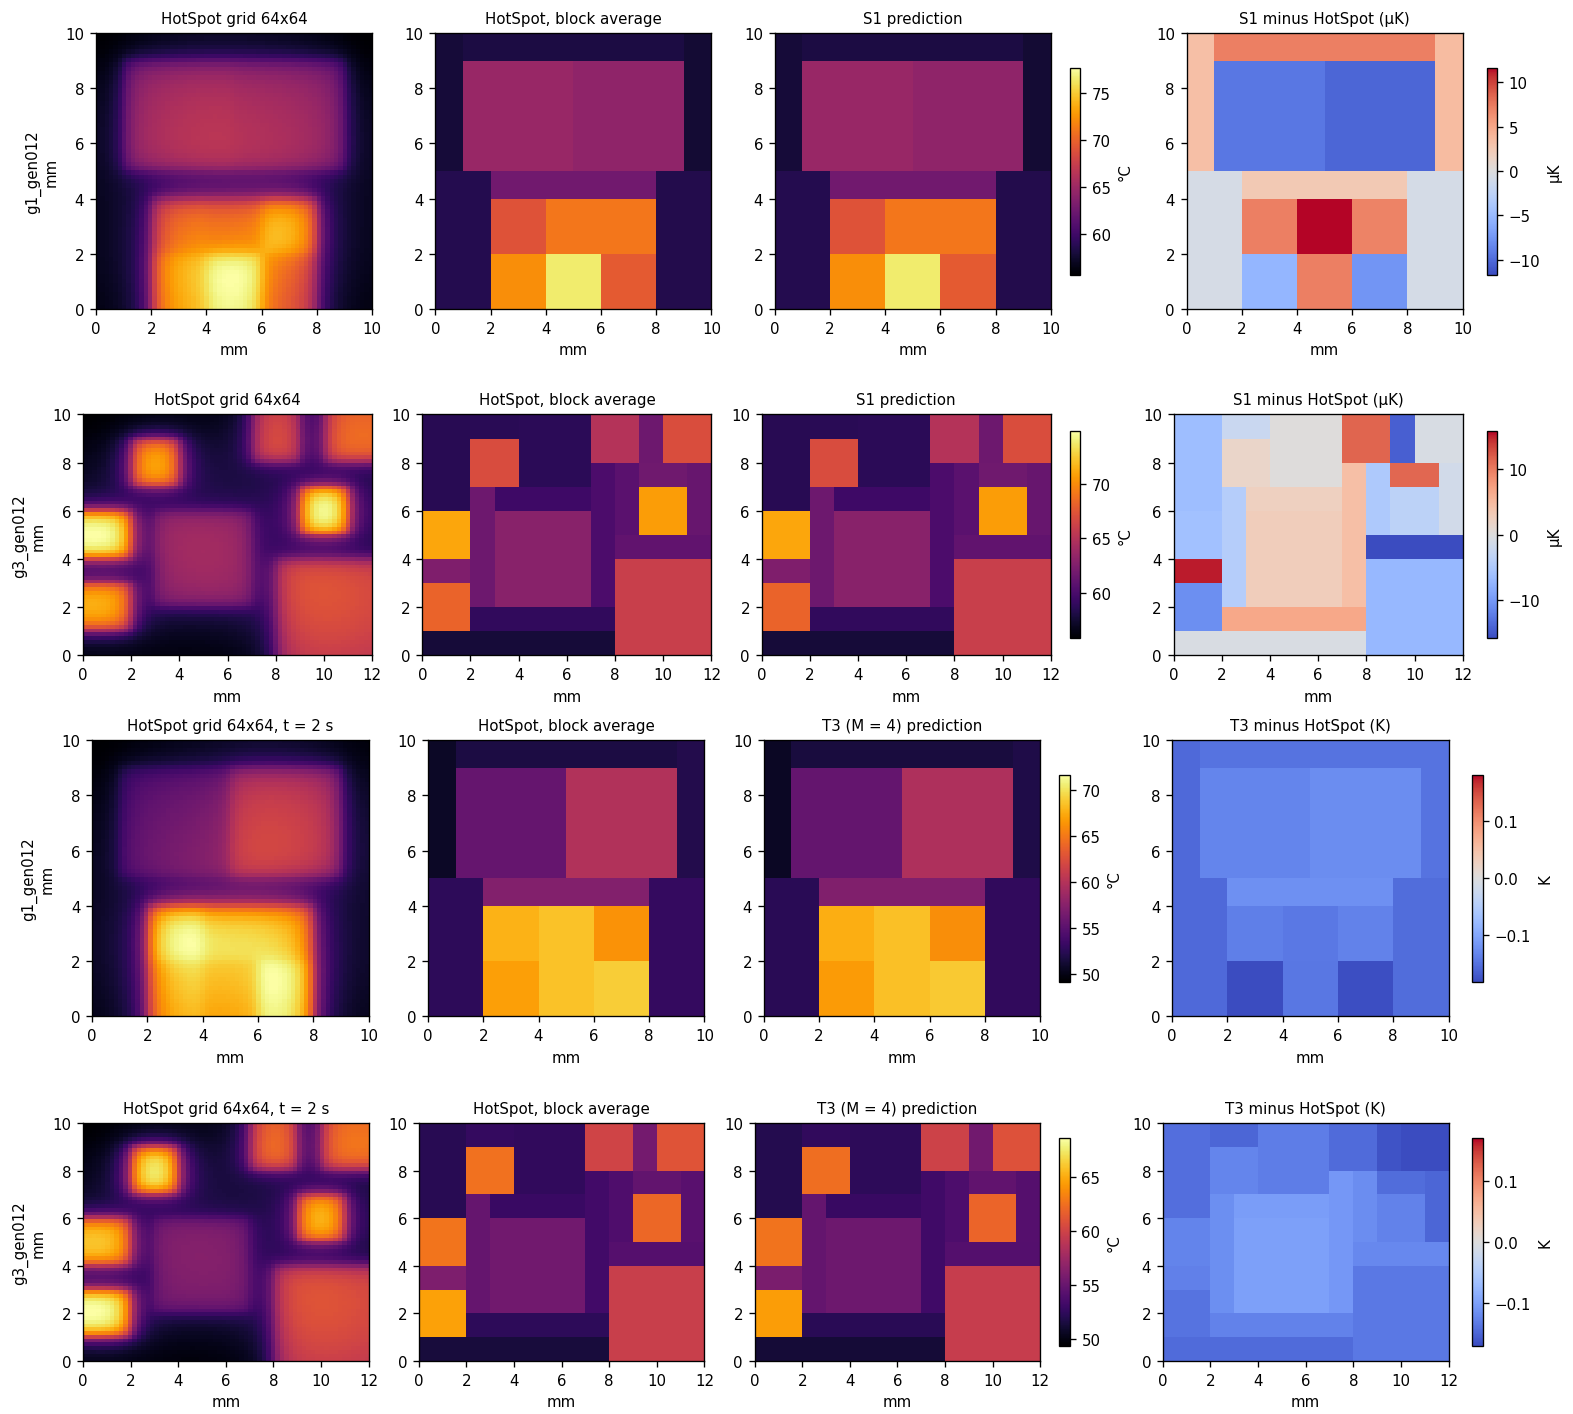
\includegraphics[width=0.85\linewidth]{extended_validation/results/report_steady_transient.png}
  \caption{Two generated floorplans. Top two rows: steady state (S1 is the influence matrix), error
  in micro-kelvin. Bottom two rows: transient at $t=2$\,s of a phase trace (T3 is the sum of four
  exponentials), error in kelvin. Columns: HotSpot's $64\times64$ map, HotSpot's block averages,
  the prediction, and prediction minus HotSpot.}
\end{figure}

%=====================================================================
\section{Robustness}
\begin{itemize}
  \item \textbf{Unusual inputs.} Power at 2--3$\times$ the maximum, bursty power, task migration
        and warm starts are all handled (transient worst 0.27--0.64\,K). A different time step from
        the calibrated one costs about 2\,K, so calibrate at the controller's time step.
  \item \textbf{Package changes.} A new ambient only needs $T_\text{amb}$ updated. A new heat sink
        needs recalibration (the old model is 4--9\,K off; 24 runs restore full accuracy).
  \item \textbf{Leakage.} Ignoring leakage costs 0.1--1\,K; a 3--4 iteration fixed-point loop
        removes it in 22--33\us\ (steady state only, as HotSpot has no transient leakage).
\end{itemize}

%=====================================================================
\section{The \texttt{ltp} tool}
Both stages are available from the command line and from Python:
{\small\begin{verbatim}
python3 -m src.ltp calibrate s4_fp001 -o model.npz      # 24 HotSpot runs, cached
python3 -m src.ltp steady    model.npz --power 20,20,8,8,8,8,8,8
python3 -m src.ltp transient model.npz --ptrace trace.ptrace -o out.ttrace
\end{verbatim}}
On one floorplan the complete model is 8{,}032\,B, a steady prediction takes 2.6\us\ and a
transient step 3.5\us.

%=====================================================================
\section{Scorecard against our targets}
\begin{center}
\small
\begin{tabular}{@{}l l c c c@{}}
\toprule
& Metric & Target & Achieved & Status \\
\midrule
Steady & Mean error per block & $\le 0.1$\,K & 0.000006\,K & met \\
& Error in the peak & $\le 0.2$\,K & 0.00003\,K & met \\
& Hottest core right & $\ge 99\,\%$ & 100\,\% & met \\
& Time per prediction & $\le 20$\us & 2.6\us & met \\
& Model size & $\le 5$\,kB & 464--928\,B & met \\
& Calibration runs & $\le 9$ & 8 (4\,s) & met \\
\midrule
Transient & Mean error over a trace & $\le 0.5$\,K & 0.06--0.09\,K & met \\
& Error in the peak & $\le 1$\,K & 0.27--0.30\,K & met \\
& Hottest core right & $\ge 95\,\%$ & 96\,\% (worst floorplan) & met \\
& Time per step & $\le 50$\us & 3.1\us & met \\
& Model size & $\le 50$\,kB & 3.7--4\,kB & met \\
& Calibration time & $\le 2$\,min wall & $\approx 2.75$\,min & slightly over \\
\bottomrule
\end{tabular}
\end{center}

%=====================================================================
\section{Verification approach}
\begin{enumerate}
  \item Keep calibration and test data strictly separate.
  \item Stress-test beyond nominal conditions.
  \item Unit tests for \texttt{ltp}; every HotSpot run cached with its command, configuration and
        git commit; one script, README and results folder per experiment.
\end{enumerate}

%=====================================================================
\section{What went as planned, and what deviated}
All must-have deliverables were completed. The main deviations:
\begin{center}
\small
\begin{tabular}{@{}p{3cm} p{4.3cm} p{7.7cm}@{}}
\toprule
Item & Planned & Done, and why \\
\midrule
HotSpot build & Precision patch & Also faster transients and a memory-leak fix: long traces were impractical or crashed. \\
Dataset & Our synthetic floorplans & The 23 given floorplans as the main set, plus 52 generated in the same styles. \\
Hot spots & One hottest cell per core & Several candidate cells: the hot spot moves. \\
Timing & One idle machine & One laptop, partly shared with HotSpot jobs. \\
\bottomrule
\end{tabular}
\end{center}

%=====================================================================
\section{Limitations}
\begin{itemize}
  \item All results are against HotSpot, not silicon measurements.
  \item Block-level models do not show hot spots inside a block, except through the candidate-cell
        model.
  \item Leakage was tested in steady state only.
  \item A model is tied to its package: a new heat sink needs recalibration.
\end{itemize}

%=====================================================================
\section{Learnings and future scope}
\textbf{Learnings.}
\begin{enumerate}
  \item HotSpot is linear without leakage, so a matrix predictor can be exact.
  \item Calibration is cheap (8 runs, 4\,s) and essential (0.5--2.7\,K without it): position
        matters, not just core type.
  \item Core averages hide hot spots 3--9\,K hotter, and the hot spot moves.
  \item Heat moves on time scales from 1\,ms to 8\,s: one time constant fails, four suffice.
  \item Planned step runs beat fitting a recorded trace.
\end{enumerate}

\textbf{Future scope.} Correcting a heat-sink change without new runs; leakage in transients;
using the predictor inside a DTM controller; calibration from real sensor data.

%=====================================================================
\section{Presentation feedback}
Feedback received during the presentation, and whether it was incorporated.
\begin{center}
\small
\begin{tabular}{@{}p{0.6cm} p{6.5cm} p{2.2cm} p{5.2cm}@{}}
\toprule
\# & Feedback & Incorporated? & Action taken / reason \\
\midrule
1 & \todo{feedback} & \todo{yes/no} & \todo{what was changed, or why not} \\
2 & & & \\
3 & & & \\
\bottomrule
\end{tabular}
\end{center}

%=====================================================================
\section{Submission contents and how to run}
\begin{itemize}
  \item \texttt{reports/}: this report and the slides (PDF and \LaTeX\ source).
  \item \texttt{src/}: implementation (\texttt{sim/} HotSpot tooling, \texttt{ltp/} predictor).
  \item \texttt{experiments/}: one folder per experiment with \texttt{run.py}, README and results.
  \item \texttt{tests/}, \texttt{setup/}, \texttt{configs/}, \texttt{data/}: unit tests, HotSpot
        patches and build script, configurations, floorplans.
  \item \texttt{README\_SETUP.md}: setup and run instructions; \texttt{docs/guide.html}: a guide
        to every experiment.
\end{itemize}
Inside WSL, from the repository root:
{\small\begin{verbatim}
bash setup/build_hotspot_ltp.sh                 # one time: build the patched HotSpot
python3 tests/test_models.py                    # unit tests
bash experiments/run.sh <experiment folder>     # run one experiment
\end{verbatim}}

%=====================================================================
\section{LLM assistance disclosure}
LLMs were used to understand HotSpot, for literature review to select appropriate models, to
generate floorplans, to write calibration and testing scripts, and to create this document
using \LaTeX.

%=====================================================================
\begin{thebibliography}{9}\small
\bibitem{hotspot} W.~Huang et al., ``HotSpot: A Compact Thermal Modeling Methodology for
  Early-Stage VLSI Design,'' \emph{IEEE TVLSI} 14(5):501--513, 2006.
\bibitem{hotspot4} W.~Huang et al., ``An Improved Block-Based Thermal Model in HotSpot 4.0 with
  Granularity Considerations,'' WDDD 2007.
\bibitem{matex} S.~Pagani, J.-J.~Chen, M.~Shafique, J.~Henkel, ``MatEx: Efficient Transient and
  Peak Temperature Computation for Compact Thermal Models,'' DATE 2015.
\bibitem{sharifi08} S.~Sharifi, C.~Liu, T.~S.~Rosing, ``Accurate Temperature Estimation for
  Efficient Thermal Management,'' ISQED 2008.
\bibitem{blurring} A.~Ziabari et al., ``Power Blurring: Fast Static and Transient Thermal Analysis
  Method for Packaged Integrated Circuits and Power Devices,'' \emph{IEEE TVLSI} 22(11):2366--2379,
  2014.
\bibitem{coskun} A.~K.~Coskun, T.~S.~Rosing, K.~C.~Gross, ``Utilizing Predictors for Efficient
  Thermal Management in Multiprocessor SoCs,'' \emph{IEEE TCAD} 28(10), 2009.
\bibitem{singla} G.~Singla, G.~Kaur, A.~K.~Unver, U.~Y.~Ogras, ``Predictive Dynamic Thermal and
  Power Management for Heterogeneous Mobile Platforms,'' DATE 2015.
\end{thebibliography}

\end{document}
